\documentclass[12pt]{beamer}
%\documentclass[20pt,handout]{beamer}
\usetheme{Darmstadt}
\usepackage{graphicx}
\usepackage[german]{babel}
\usepackage[T1]{fontenc}
\usepackage[utf8]{inputenc}
\usepackage{tikz}
\setbeamertemplate{footline}[frame number]

\newcommand{\cc}[1]{\includegraphics[height=4mm]{img/#1.png}}
\usepackage{ifthen}
\newcommand{\license}[2][]{\\#2\ifthenelse{\equal{#1}{}}{}{\\\scriptsize\url{#1}}}
\usepackage{textcomp}

\pgfdeclareimage[height=.6cm]{c3d2logo}{./img/c3d2.pdf} 


\pgfdeclarelayer{foreground}
\pgfsetlayers{main,foreground}
\logo{\pgfputat{\pgfxy(-1,0)}{\pgfbox[center,base]{\pgfuseimage{c3d2logo}}}}


\title{Chaos macht Schule}
\author{\small Marius Melzer \& Johannes Steinmetz\\\large Chaos Computer Club Dresden}
\date{\today}

\begin{document}
\maketitle


\begin{frame}
  \frametitle{Einleitung}
  \begin{figure}
    
\includegraphics[height=0.7\textheight]{img/fingerabdruck.jpg}
  \end{figure}
\end{frame}


\section{Einleitung}
\begin{frame}
    \frametitle{Chaos Computer Club}
    \begin{itemize}
      \item<1-> Chaos Computer Club Dresden (\url{http://c3d2.de})
          \note{}
      \item<2-> Datenspuren: Herbst 2014 \url{http://datenspuren.de}
      \item<3-> Podcasts (\url{http://pentamedia.de})
      \item<4-> Chaos macht Schule
    \end{itemize}
\end{frame}

\begin{frame}
  \frametitle{Einleitung}
  \begin{figure}
    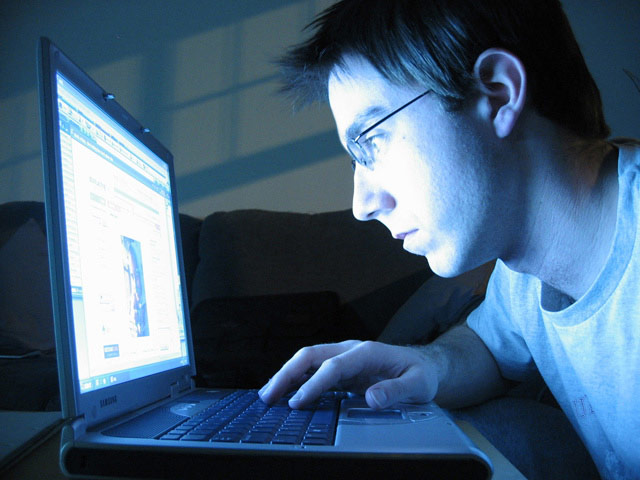
\includegraphics[height=0.7\textheight]{img/internet_user1.jpg}
  \end{figure}
\end{frame}

\begin{frame}
  \frametitle{Einleitung}
  \begin{figure}
    
\includegraphics[height=0.7\textheight]{img/internet_user3.jpg}
  \end{figure}
\end{frame}

\begin{frame}
  \frametitle{Einleitung}
  \begin{figure}
    
\includegraphics[height=0.7\textheight]{img/internet_user4.jpg}
  \end{figure}
\end{frame}

\begin{frame}
  \frametitle{Einleitung}
  \begin{figure}
    
\includegraphics[height=0.7\textheight]{img/internet_user2.jpg}
  \end{figure}
\end{frame}

\begin{frame}
  \frametitle{Gliederung}
  \begin{itemize} \Large
    \item Grundlagen des Internets
    \item Verfolgung im Internet
    \item Soziale Netzwerke
    \item Digitaler Selbstschutz
  \end{itemize}
\end{frame}

\section{Grundlagen des Internets}

\begin{frame}
    \frametitle{Wie kommunizieren wir im Internet?}
    \begin{center}
      
\includegraphics[width=7cm]{img/direkt.png}
    \end{center}
\end{frame}

\begin{frame}
    \frametitle{Wie kommunizieren wir im Internet?}
    \begin{center}
      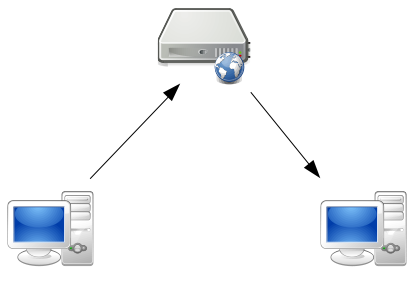
\includegraphics[height=5cm]{img/c-s.png}
    \end{center}
\end{frame}

\begin{frame}
    \frametitle{Zwischenstationen}
    \begin{center}
      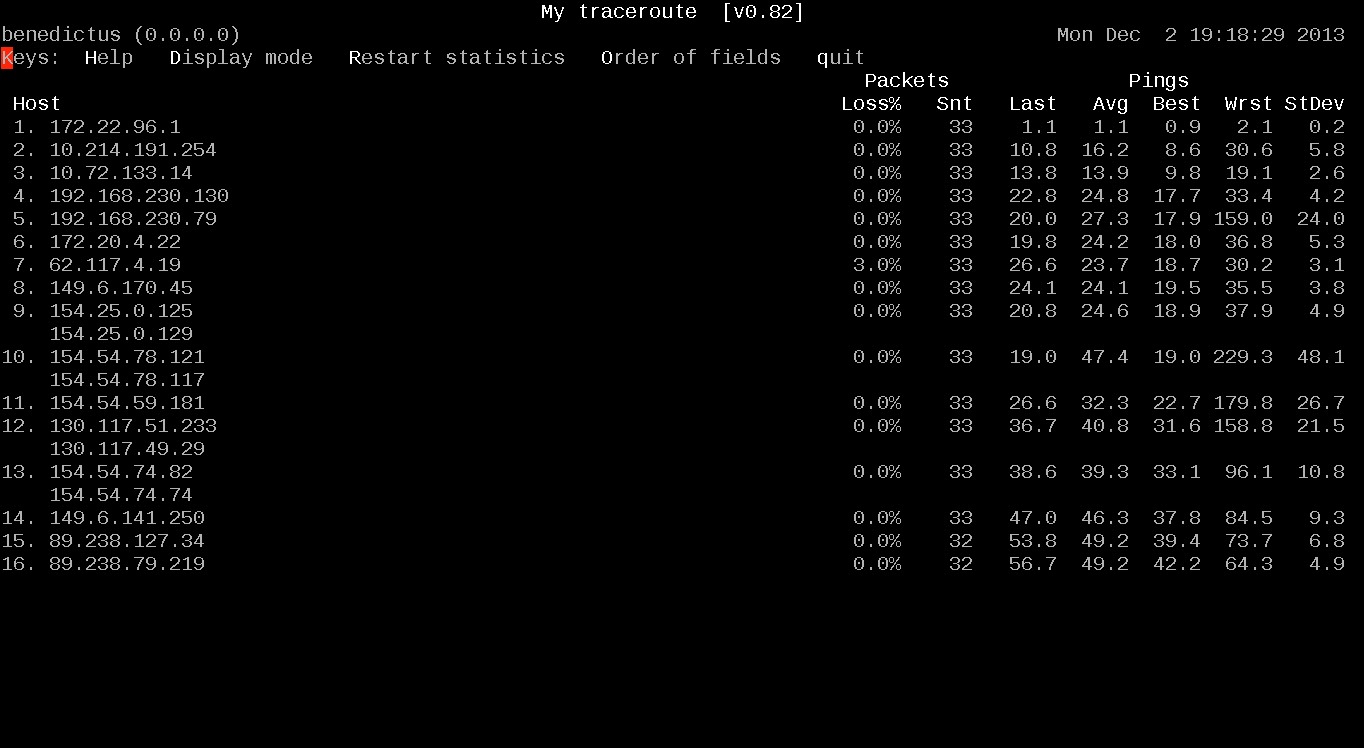
\includegraphics[height=5cm]{img/mtr.png}
    \end{center}
\end{frame}

\begin{frame}
	\frametitle{Grundlagen des Internets}
	\begin{center}
		\begin{itemize}
			\item<1-> Alle Internetteilnehmer haben eindeutige IP Adresse
			\item<2-> DNS → Telefonbuch für das Internet
		\end{itemize}
	\end{center}
\end{frame}

\begin{frame}
  \frametitle{Grundlagen des Internets}
  \begin{figure}
    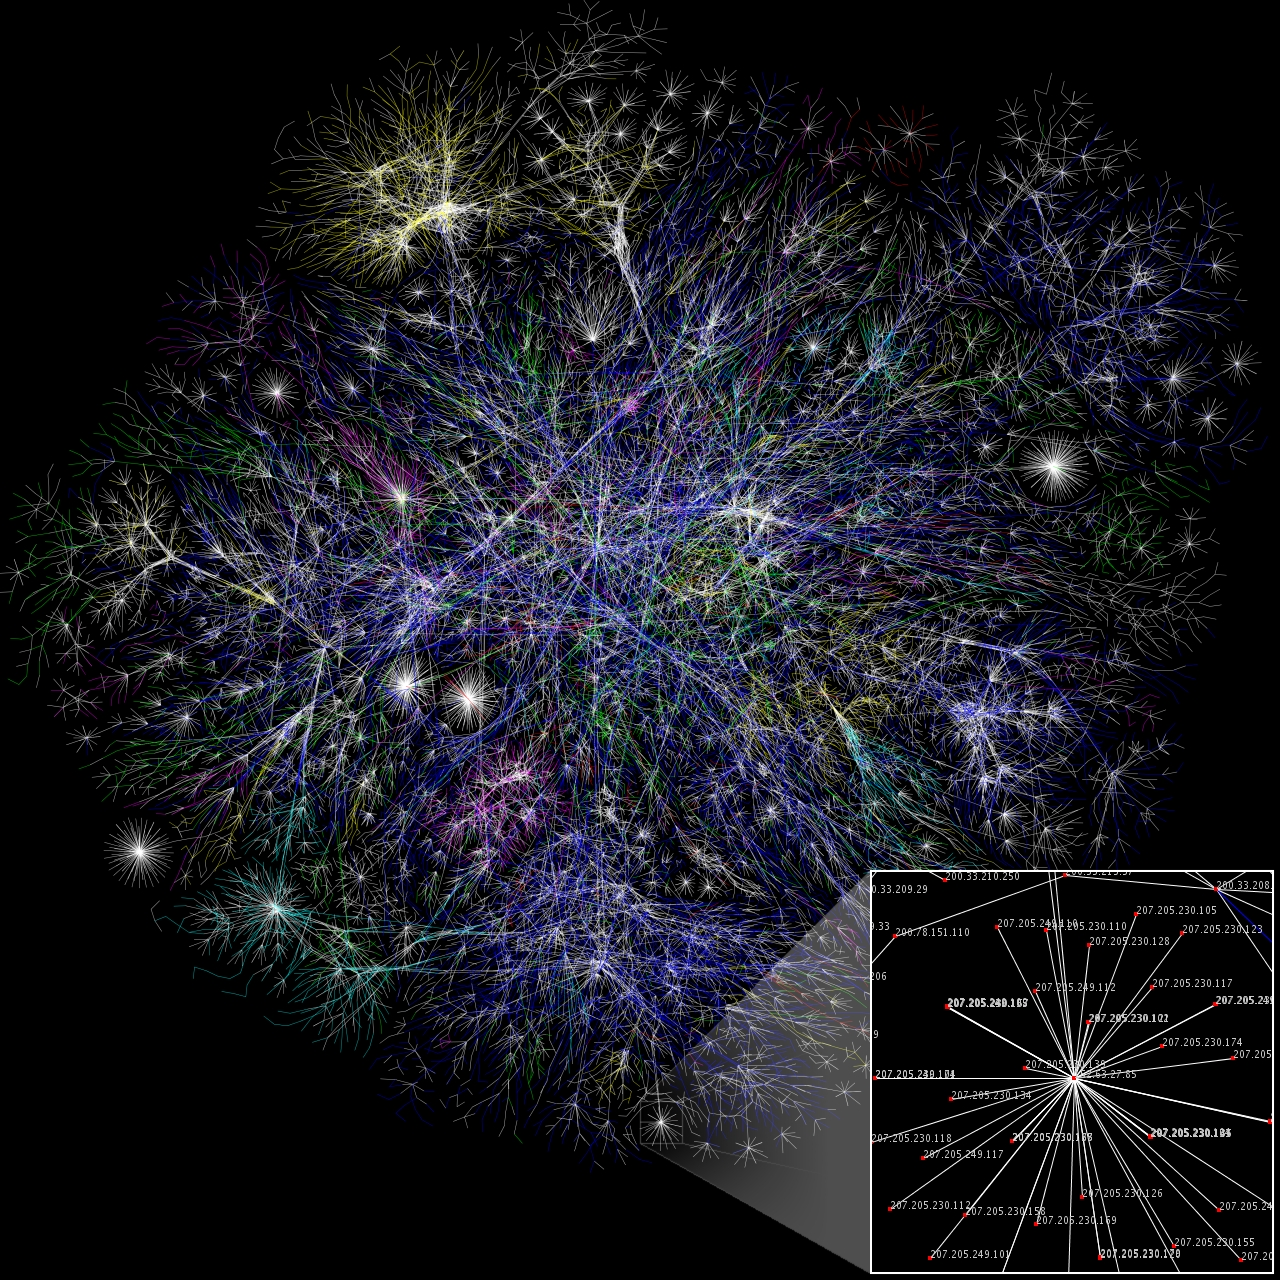
\includegraphics[height=0.85\textheight]{img/internet_map.jpg}
  \end{figure}
\end{frame}

\begin{frame}
  \frametitle{Ewiger Speicher}
  \begin{center} \Large
   Das Internet vergisst nichts!\\
	  \onslide<2->{
   \small{…zumindest nicht wenn man es gern hätte.}}
  \end{center}
\end{frame}

\begin{frame}
  \frametitle{Vor wem kann man sich schützen wollen?}
 \begin{itemize}
	\item <2-> Staaten und Geheimdienste
	\item <3-> Firmen und Dienstanbieter
 	\item <4-> Lehrer, Eltern, Freunde, Böse Menschen
 \end{itemize} 
  %FIXME \onslide<5> \includegraphics[height=.4\textheight]{img/FIXME
\end{frame}

\section{-gegenüber dem Staat}
\subsection{}

\begin{frame}
	\frametitle{Stasi vs NSA}
	\begin{center}
		\texttt{ „Wir wissen z.B., dass es nicht so ist, wie bei der Stasi und dem KGB, dass es dicke Aktenbände gibt, wo unsere Gesprächsinhalte alle aufgeschrieben und schön abgeheftet sind. Das ist es nicht.“}
	\end{center}
	\begin{flushright}
		\textit{Bundespräsident Gauck zur NSA-Überwachung}
	\end{flushright}
\end{frame}

\begin{frame}
    \frametitle{Stasi vs. NSA}
    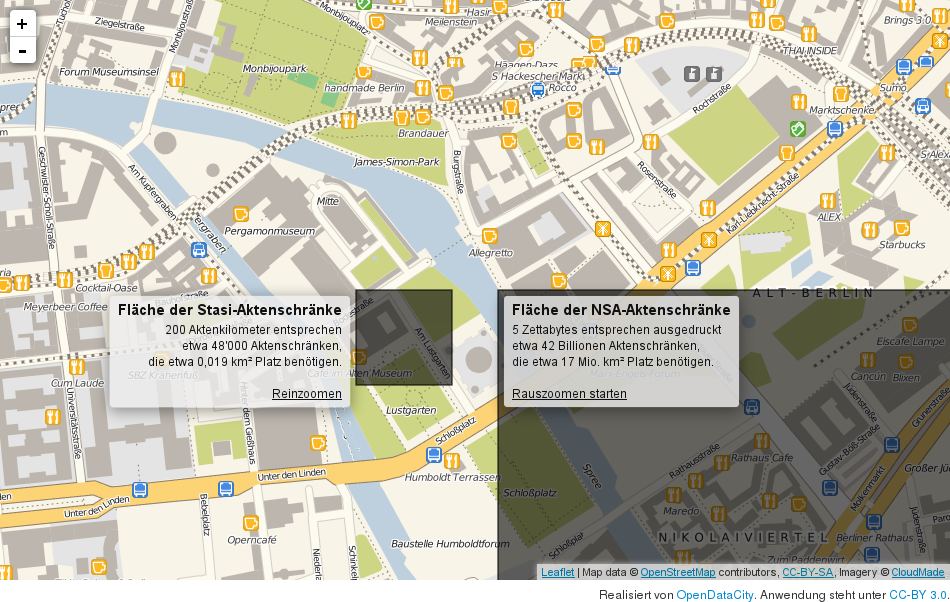
\includegraphics[height=0.7\textheight]{img/akten1.png}
\end{frame}

\begin{frame}
    \frametitle{Stasi vs. NSA}
    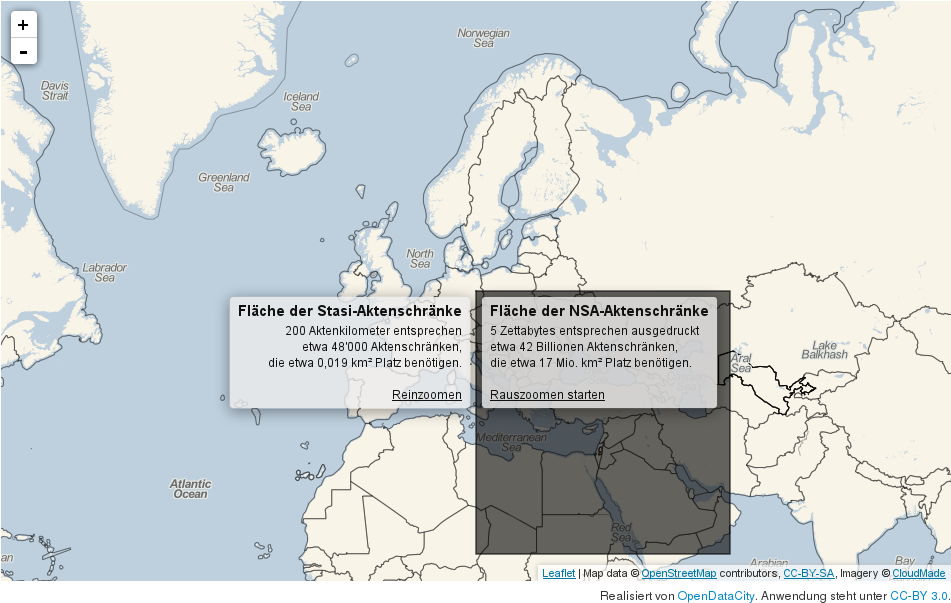
\includegraphics[height=0.7\textheight]{img/akten2.png}
\end{frame}

\begin{frame}
  \frametitle{Verschlüsselung}
  \begin{center} \Large
  Verschlüsselung\\
  \onslide<2->{… eigenes Thema}
  \begin{itemize}
  	\item <3-> SSL \& TLS
	\item <3-> Ende zu Ende (GPG)
  \end{itemize}
  \end{center}
\end{frame}

\section{-gegenüber Firmen}
\subsection{}

\begin{frame}
  \frametitle{Geschäftsmodelle}
  \begin{itemize}
    \item Womit verdienen folgende Firmen ihr Geld?
      \begin{itemize}
        \item<2-> Karstadt
        \item<3-> Amazon
        \item<4-> Ebay
        \item<5-> Facebook
      \end{itemize}
      \onslide<6-> Werbung verkauft sich personalisiert besser -> Personalisieren durch Tracking
  \end{itemize}
\end{frame}

\begin{frame}
  \frametitle{}
  \begin{center} \Large
   Für wieviel Geld würdet ihr eure (Profil-)Daten verkaufen?
  \end{center}
\end{frame}


\begin{frame}
  \frametitle{Kunde oder Produkt?}
  \begin{figure}
    
\includegraphics[height=0.7\textheight]{img/business_pigs.jpg}
  \end{figure}
\end{frame}

\begin{frame}
  \frametitle{Beispiel: Soziale Netzwerke}

  \begin{itemize}
    \item Was haben soziale Netzwerke von euch?\\(am Bsp. von Facebook)
      \begin{itemize}
        \item<2-> 82\% Einnahmen aus Werbung
        \item<3-> 30\% Anteil an "`Facebook-Einkäufen"'
        \item<4-> durchschnittlich 1€/Profil
        \item<5-> "`Poweruser"'-Profile deutlich mehr
        \item<6-> => Mehr Werbegewinn durch personalisierte Werbung
      \end{itemize}
  \end{itemize}
\end{frame}

\begin{frame}
  \frametitle{Möglichkeiten der Dienstanbieter}
      \begin{itemize}
        \item<1-> Referrer
        \item<2-> Cookies
        \item<3-> Zählpixel
        \item<4-> Like-Buttons, Facebook-Login, Apps + Spiele
      \end{itemize}
\end{frame}

\begin{frame}
  \frametitle{Gegenmaßnahmen}
      \begin{itemize}
        \item<2-> Einstellungen im Browser
        \item<3-> Ghostery
        \item<4-> Adblock
      \end{itemize}
\end{frame}

\begin{frame}
  \frametitle{weitergehende Erkennung}
  \begin{center} \Large
    https://panopticlick.eff.org/
  \end{center}
\end{frame}

%FIXME Folie mit Tor Browser

\begin{frame}
  \frametitle{Alternativen?}
  \begin{center} \Large
    Suchmaschinen
  \end{center}
\end{frame}

\begin{frame}
  \frametitle{Soziale Netzwerke}

  \begin{itemize}
    \item Wer ist in welchem sozialen Netzwerk?
      \begin{itemize}
        \item SchülerVZ
        \item SchülerCC
        \item Facebook
        \item Google+
        \item ICQ/MSN/Jabber
        \item Flickr
        \item Last.fm / Jamendo
        \item Youtube
        \item weitere?
      \end{itemize}
  \end{itemize}
\end{frame}

\begin{frame}
  \frametitle{Soziale Netzwerke}

  \begin{center} \Large
     Was bieten soziale Netzwerke?
  \end{center}
\end{frame}

\begin{frame}
  \frametitle{Soziale Netzwerke}

  \begin{center} \Large
   Alternativen zu Facebook und co.
  \end{center}
\end{frame}



\begin{frame}
  \frametitle{Soziale Netzwerke}
  \begin{center} \Large
     Datensparsamkeit 
     \begin{itemize}
     	\item Pseudonymität
	\item „Daten“ ausdenken 
	\item Veröffentlichungsbewustsein
     \end{itemize}
  \end{center}
\end{frame}

\section{-gegenüber anderen Menschen}
\subsection{}

\begin{frame}
	\frametitle{Probleme}

	\begin{itemize}
		\item Schutz vor „Neugierigen“
			\begin{itemize}
				\item Datenschutzeinstellungen
			\end{itemize}
		\item Identitätsdiebstahl
			\begin{itemize}
				\item Profilklau
				\item Kopie des Profils
			\end{itemize}
	\end{itemize}
\end{frame}

\begin{frame}
  \frametitle{Passwortsicherheit}
  \begin{itemize}
    \item (nCuAj.§Tsm!f
    \item IchLiebeDich
    \item .§)=")=`
    \item 123456
    \item alkmgfksjr
    \item Mks?o/.u,ePsw!
  \end{itemize}
\end{frame}

\begin{frame}
  \frametitle{Soziale Netzwerke}

  \begin{figure}
    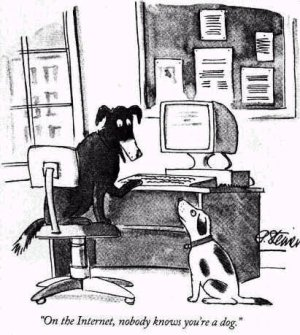
\includegraphics[height=0.7\textheight]{img/internet_dog.jpg}
    \license[http://en.wikipedia.org/wiki/File:Internet\_dog.jpg]{\copyright Image from New Yorker cartoon by Peter Steiner.}
  \end{figure}
\end{frame}

\begin{frame}
  \frametitle{Soziale Netzwerke}

  \begin{center} \Large
    Identitätsklau - aus Sicht des Angreifers
  \end{center}
\end{frame}

\begin{frame}
  \frametitle{Datenschutz}

  \begin{itemize}
    \item Wem sollte man preisgeben/posten (und was eher nicht)?
      \begin{itemize}
        \item<2-> "`Roadkill"' von Entertainment for the Braindead ist ein cooles Album
        \item<3-> Jan Müller geht am Donnerstag, den 07.06.2012 zum Poetry Slam in der Scheune
        \item<4-> Ich bin heut' echt gut drauf!
        \item<5-> Ute Meyer war mit Carolin Wittich und Frederik Ulm am Samstag abend im Schillergarten Fußball gucken und ist danach mit Michael Müller nach Hause gefahren
        \item<6-> Meine Lehrerin ist voll doof!
      \end{itemize}
  \end{itemize}
\end{frame}

\begin{frame}
  \frametitle{Datenschutz}

  \begin{itemize}
    \item Datenschutz anderer Personen respektieren:
      \begin{itemize}
        \item<2->Bilder taggen
        \item<3->Emailadressen importieren
        \item<4->Angeben, mit wem man etwas unternimmt
      \end{itemize}
  \end{itemize}
\end{frame}

\begin{frame}
  \frametitle{Datenschutz}

  \begin{itemize}
    \item Eigenschutz
      \begin{itemize}
        \item<2->Moderation von Posts
        \item<3->Freunde auf Fehlverhalten hinweisen
        \item<4->Aufpassen was und wieviel man preisgibt
      \end{itemize}
  \end{itemize}
\end{frame}

\begin{frame}
  \frametitle{Diskussion}
  \begin{center}
    {\Large Diskussion}\\
    \vspace{5mm} 
    \href{https://github.com/c3d2/cms-nsa}{Folien}: \href{https://creativecommons.org/licenses/by-sa/4.0/}{\cc{by-sa}} Chaos Computer Club Dresden \\
    \vspace{4mm}
    https://c3d2.de
    Kontakt: schule@c3d2.de
  \end{center}
\end{frame}
\end{document}
